This section validates the environment mechanics and quantifies the
optimality gap available to future learned policies. Three
deterministic greedy heuristics and a full-information optimum are evaluated across four benchmark portfolio
configurations of increasing structural complexity. Each configuration
isolates a specific mechanic of the environment --- progress dynamics,
advance payment timing, termination risk, and multi-project
coordination --- enabling precise attribution of each heuristic's
failure mode. All episodes are executed through the Gymnasium
environment described in Section~\ref{sec:problem}, with the SQLite
audit ledger providing a complete per-period record of allocations,
cash-flow events, and breach flags.

% ------------------------------------------------------------
\subsection{Shared Parameters}
\label{subsec:shared_params}
% ------------------------------------------------------------

All four configurations share the contract and environment parameters
listed in Table~\ref{tab:shared_params}, fixed across every episode
and every solver so that observed performance differences are
attributable solely to configuration structure and solver policy.

\begin{table}[H]
  \centering
  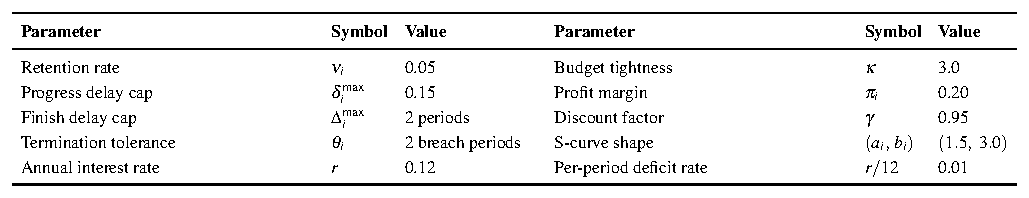
\includegraphics[width=\textwidth]{tables/shared_params.pdf}
  \caption[Configuration Shared Parameters]{Parameters shared across all benchmark configurations.}
  \label{tab:shared_params}
\end{table}

\paragraph{Duration convention.}
A project with planned duration $D_i$ executes over project-timesteps
$\tau_i \in \{0, 1, \ldots, D_i\}$, giving $D_i + 1$ active periods.
With finish delay cap $\Delta^{\max}_i = 2$, the hard deadline falls
at episode period $f_i + 2$, and each efficiency sequence has length
$D_i + 3$ entries covering all possible active periods.

\paragraph{Deduction order.}
Advance recovery is applied first to the gross milestone payment;
retention is deducted from the same gross payment independently and
in parallel. At the final milestone, any advance not yet recovered is
cleared in full and all accumulated retention is released.

% ------------------------------------------------------------
\subsection{Benchmark Configurations}
\label{subsec:configs}
% ------------------------------------------------------------

The four benchmark configurations are constructed from a common
parameter baseline (Table~\ref{tab:shared_params}) by selectively
overriding the structural dimensions listed in
Table~\ref{tab:config_axes}: project count, start-time scheme,
milestone and payment structure, and efficiency realisation. Each
override activates exactly one additional mechanic relative to the
previous configuration, so the ordering from TC-10SF-R to TC-3XMAIF-R
traces a controlled complexity ladder. Table~\ref{tab:configs}
summarises the resulting distinguishing parameters; all other fields
retain the shared defaults.

\begin{table}[H]
  \centering
  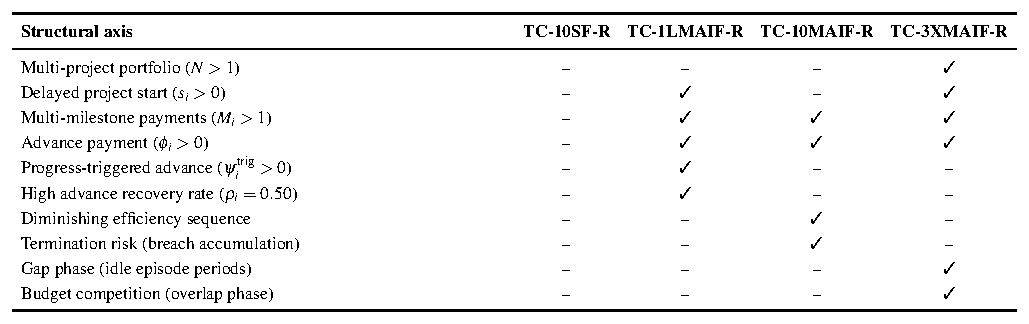
\includegraphics[width=\textwidth]{tables/config_axes.pdf}
  \caption[Complexity Structure Matrix]{Structural dimensions
    activated per benchmark configuration. Each configuration adds
    exactly one dimension over its predecessor; the first serves as
    the degenerate single-project anchor.}
  \label{tab:config_axes}
\end{table}


\paragraph{TC-10SF-R --- Isolated atom.}
One project, one non-advance milestone, no advance payment, planned
duration $D_i = 0$. The project has a single planned action at
$\tau_i = 0$ and the hard deadline falls at episode period 2.
Contract price $P_i = 120$; the single milestone carries weight
$w = 1.0$.

\paragraph{TC-1LMAIF-R --- Delayed start and progress-triggered advance.}
One project, planned start $s_i = 2$, planned duration $D_i = 3$
(four active periods: $\tau_i \in \{0,1,2,3\}$), three non-advance
milestones, advance rate $\phi_i = 0.20$ with trigger at
$\psi^{\mathrm{trig}}_i = 0.80$. The advance of
$\phi_i \times P_i = 24$ is disbursed only once cumulative progress
$EV_{i,t} \geq 0.80$ is reached. Advance recovery rate
$\rho_i = 0.50$ is the highest in the benchmark suite.
Efficiency sequence: $[0.91,\, 1.17,\, 0.83,\, 0.91,\, 1.17,\, 0.83]$.

\paragraph{TC-10MAIF-R --- Diminishing efficiency and termination risk.}
One project, planned start $s_i = 0$, planned duration $D_i = 3$,
three milestones, advance rate $\phi_i = 0.20$ disbursed at project
start ($\psi^{\mathrm{trig}}_i = 0.00$), advance recovery rate
$\rho_i = 0.20$. The efficiency sequence is monotonically decreasing:
$[0.95,\, 0.91,\, 0.55,\, 0.40,\, 0.30,\, 0.20]$. The advance of
$24$ is disbursed at $t = 0$. This configuration stress-tests the
termination mechanic as the sharp efficiency drop makes it
progressively more expensive to keep
$\delta_{i,t} \leq \delta^{\max}_i = 0.15$.

\paragraph{TC-3XMAIF-R --- Multi-project with gap and overlap.}
Three projects with heterogeneous scale
($\mathrm{BAC}_i = [100,\, 200,\, 300]$, prices $[120,\, 240,\, 360]$)
and staggered starts ($s_i = [0,\, 6,\, 7]$). Each project has
planned duration $D_i = 3$, three milestones, and advance rate
$\phi_i = 0.20$ disbursed at project start. The episode has two
structurally distinct phases: a \emph{gap phase} ($t = 4,\,5$) where
no allocations are required and the budget accumulates, and an
\emph{overlap phase} ($t = 7,\,8,\,9$) where Projects~1 and 2
compete simultaneously for the shared reserve $B_t$.

\begin{table}[H]
  \centering
  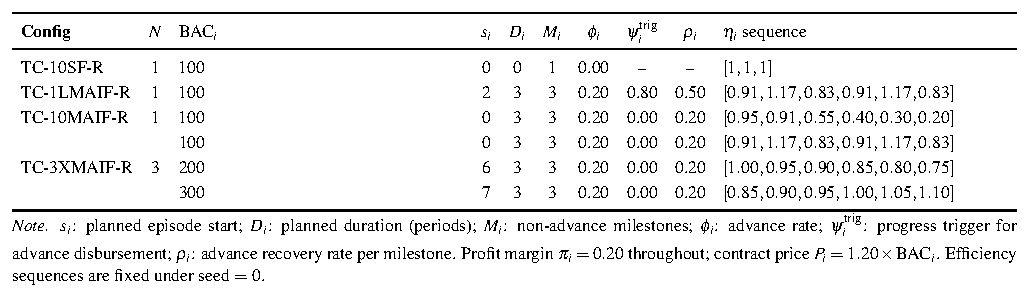
\includegraphics[width=\textwidth]{tables/configs.pdf}
  \caption[Benchmark Configurations]{Per-configuration parameter
    summary. All other fields retain the shared baseline defaults
    of Table~\ref{tab:shared_params}.}
  \label{tab:configs}
\end{table}

% ------------------------------------------------------------
\subsection{Solvers}
\label{subsec:solvers}
% ------------------------------------------------------------

Four methods are evaluated, defined formally in
Section~\ref{subsubsec:baselines}.

\textbf{Reach-Plan} ($\pi^{\mathrm{rp}}$) allocates $x^{\mathrm{rp}}_{i,t}$
to bring every active project exactly to its S-curve planned progress
each period, regardless of budget scarcity or milestone proximity.

\textbf{Catchup-T} ($\pi^{\mathrm{cu}}$) allocates the minimum spend
$x^{\mathrm{cu}}_{i,t}$ required to keep the progress delay within
$\delta^{\max}_i$ this period, preserving budget for later periods
and other projects.

\textbf{Catchup-Next-T} ($\pi^{\mathrm{cu}+1}$) pre-emptively
allocates $x^{\mathrm{cu}+1}_{i,t}$ so that the projected delay next
period also remains within $\delta^{\max}_i$, at the cost of higher
early expenditure.

\textbf{Full-information optimum} ($\pi^*$) is derived with complete
prior knowledge of all efficiency realisations $(\eta_{i,t})$, with
the efficiency sequences fixed before the episode begins. It serves as
the upper-bound reference $Z^*$ from Proposition~\ref{prop:upper_bound}.

\paragraph{Optimality verification.}
When all $\eta_{i,t}$ are known in advance, the stochastic MDP reduces
to a deterministic finite-horizon problem. The allocation action at
each active period is chosen from a small finite set: at the
project level, the feasible choices are to target the current-period
catch-up amount, the next-period catch-up amount, the milestone
completion amount, or zero. With three projects spanning at most two
concurrent active periods and an episode horizon of $T = 13$, the
Cartesian product of per-period action sets is fully enumerable in
polynomial time. Each candidate allocation sequence is evaluated by
executing the environment's deterministic transition kernel forward
from $t = 0$, applying the FIDIC cash-flow mechanics exactly as
specified in Section~\ref{sec:problem}, and recording the cumulative
discounted return $G = \sum_{t} \gamma^t \Delta B_t$. The proposed
$\pi^*$ sequence is confirmed to be optimal: no alternative allocation
sequence over the same fixed efficiency realisations yields a higher
$G$. The enumeration therefore constitutes the formal basis for
treating $\pi^*$ as the performance ceiling across the four
configurations studied here.

All four methods are evaluated under seed $= 0$ with fixed
custom-ordinal efficiency sequences, ensuring exact reproducibility
across runs and solvers.

% ------------------------------------------------------------
\subsection{Traceback over the Optimised Solution}
\label{subsec:traceback}
% ------------------------------------------------------------

This subsection decomposes the full-information optimum $\pi^*$ on
TC-3XMAIF-R into its period-by-period mechanics. TC-3XMAIF-R is
chosen because it is the only configuration in which $\pi^*$ achieves
a positive NPV while every greedy heuristic records a loss; the
traceback therefore identifies the exact decisions that convert a
complex multi-project portfolio from loss-making to profitable.

The episode runs from $t = 0$ to $t = T = 13$ and decomposes into
four structural phases:

\begin{enumerate}
  \item \textbf{Pre-gap} ($t = 0$--$3$): Project~0 is the sole active
        project. The optimum front-loads allocation into
        high-efficiency periods to certify milestones early and
        accumulate the budget reserve ahead of the gap.
  \item \textbf{Gap} ($t = 4$--$5$): No project is active; the
        portfolio balance accrues interest, net of any deficit charge
        if the balance is negative. The gap is an artefact of the
        staggered-start design and rewards policies that avoid entering
        it with a deficit.
  \item \textbf{Ramp-up and first overlap} ($t = 6$--$7$): Project~1
        starts at $t = 6$ and Project~2 at $t = 7$, triggering advance
        outflows of $48$ and $72$ respectively. The optimum sequences
        these disbursements to preserve a positive balance through both.
  \item \textbf{Full overlap} ($t = 8$--$9$) and \textbf{tail}
        ($t = 10$--$13$): Projects~1 and 2 compete for the shared
        reserve. The optimum exploits known efficiency sequences to
        allocate first to whichever project yields the higher marginal
        milestone return per unit of expenditure.
\end{enumerate}

\paragraph{Gantt timeline.}
Figure~\ref{fig:gantt_optimal} shows the planned and realised activity
intervals for all three projects under $\pi^*$, with milestone
certification events annotated.

\begin{figure}[H]
  \centering
  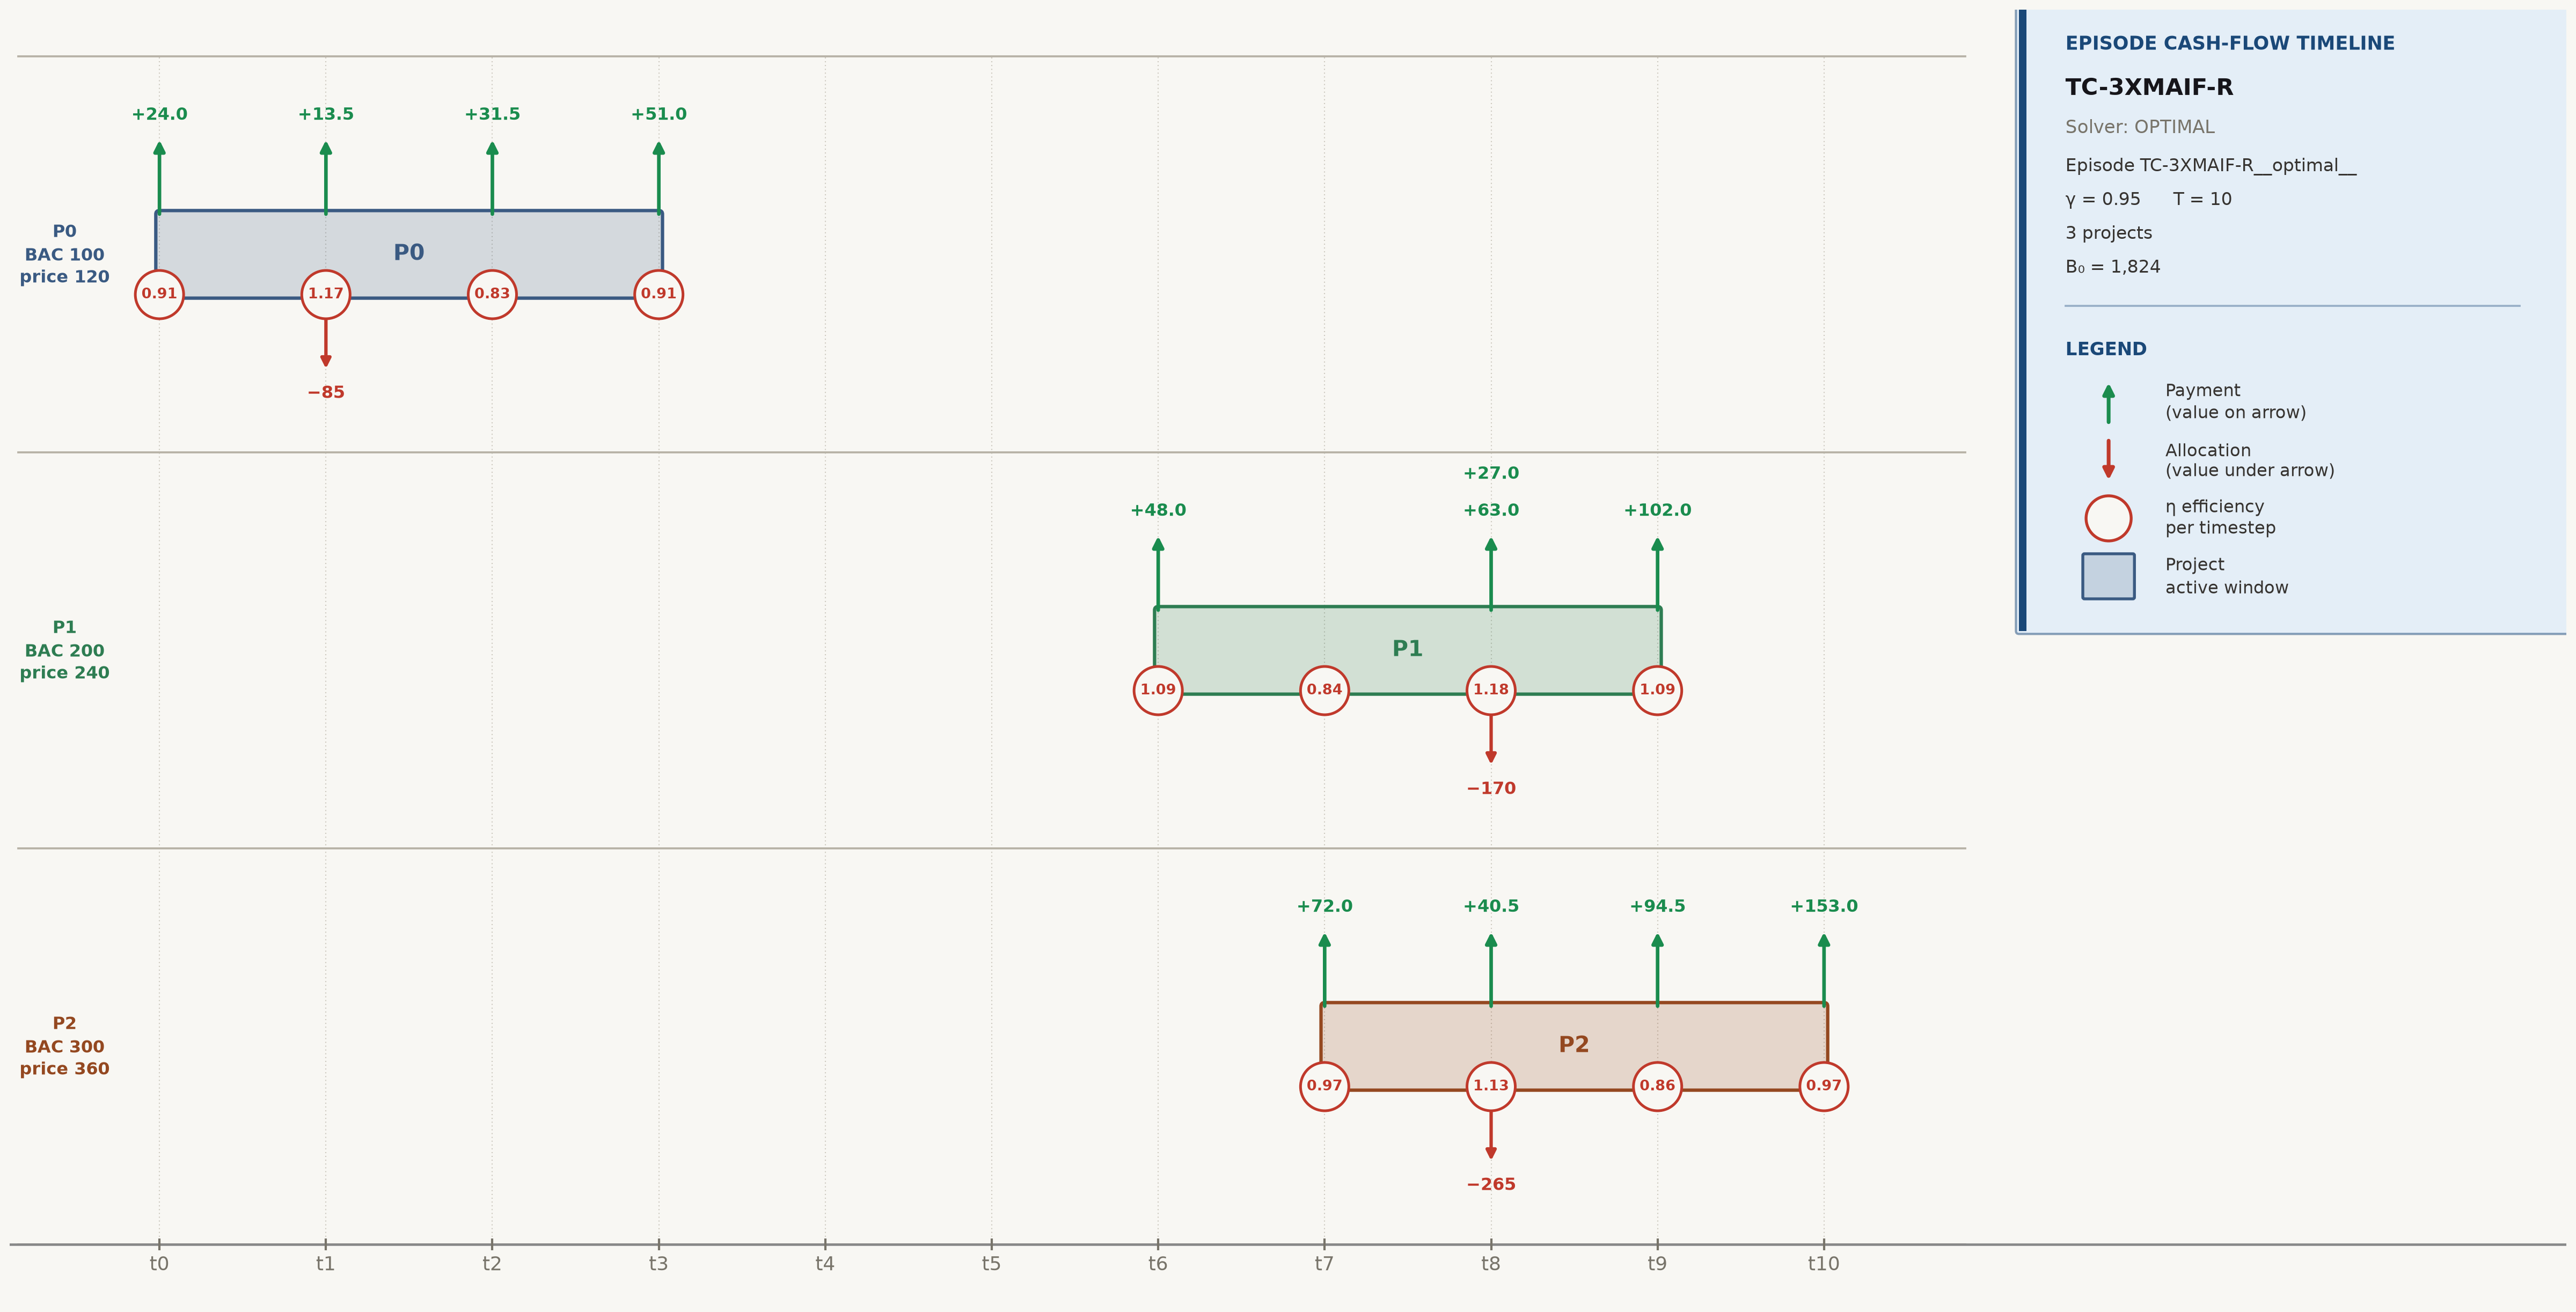
\includegraphics[width=\textwidth]{figures/gantt_optimal.png}
  \caption[Optimal Gantt Timeline]{Planned and realised activity
    intervals for the three-project configuration under the
    full-information optimum $\pi^*$.}
  \label{fig:gantt_optimal}
\end{figure}

\paragraph{Cost baseline and EVM curves.}
Figure~\ref{fig:cost_baseline_three} plots the Planned Value (PV),
Earned Value (EV), and Actual Cost (AC) curves for each project under
$\pi^*$. The cost baseline confirms that the optimum respects the
S-curve planned expenditure profile during high-efficiency periods and
intentionally under-spends during low-efficiency periods, accepting a
controlled progress delay rather than incurring wasteful expenditure.

\begin{figure}[H]
  \centering
  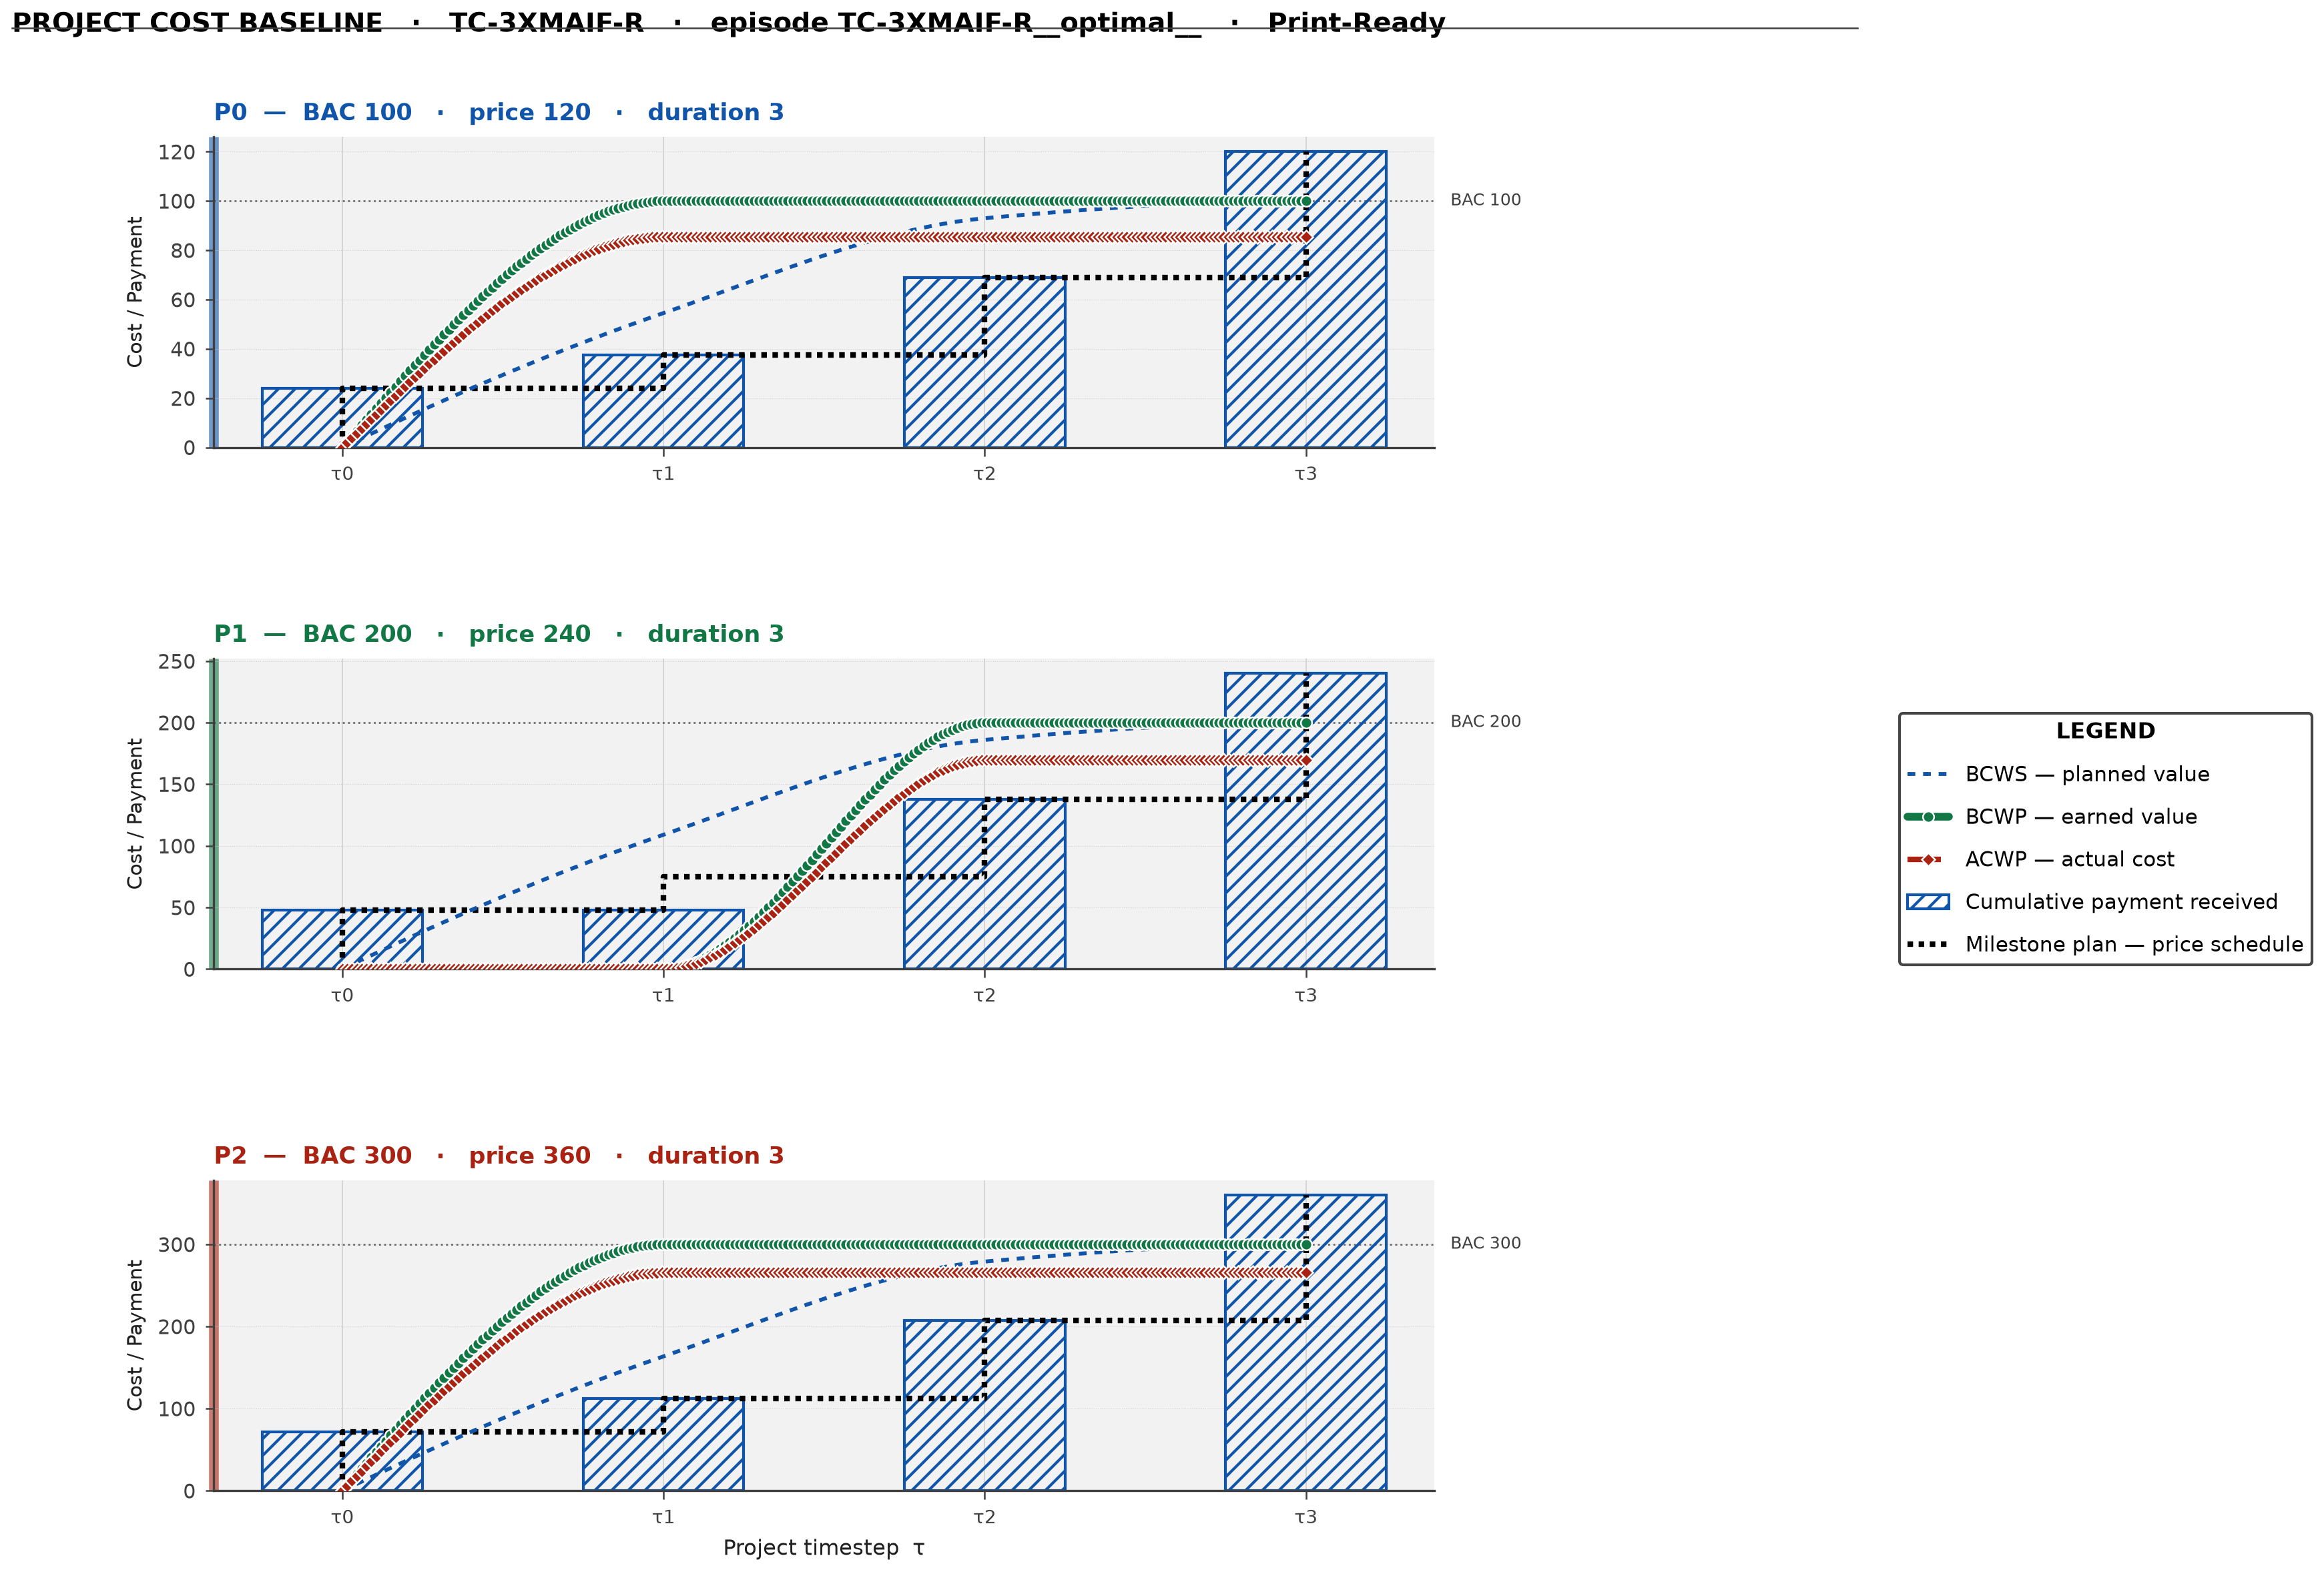
\includegraphics[width=\textwidth]{figures/01c_cost_baseline_E.png}
  \caption[Project Cost Baselines]{EVM curves under the
    full-information optimum $\pi^*$.}
  \label{fig:cost_baseline_three}
\end{figure}

\paragraph{Net cash-flow diagram.}
Figure~\ref{fig:cashflow_optimal} disaggregates the period-by-period
cash-flow into four components: allocation outflows, advance
disbursements, milestone inflows (net of recovery and retention
deductions), and the running portfolio balance $B_t$.

\begin{figure}[H]
  \centering
  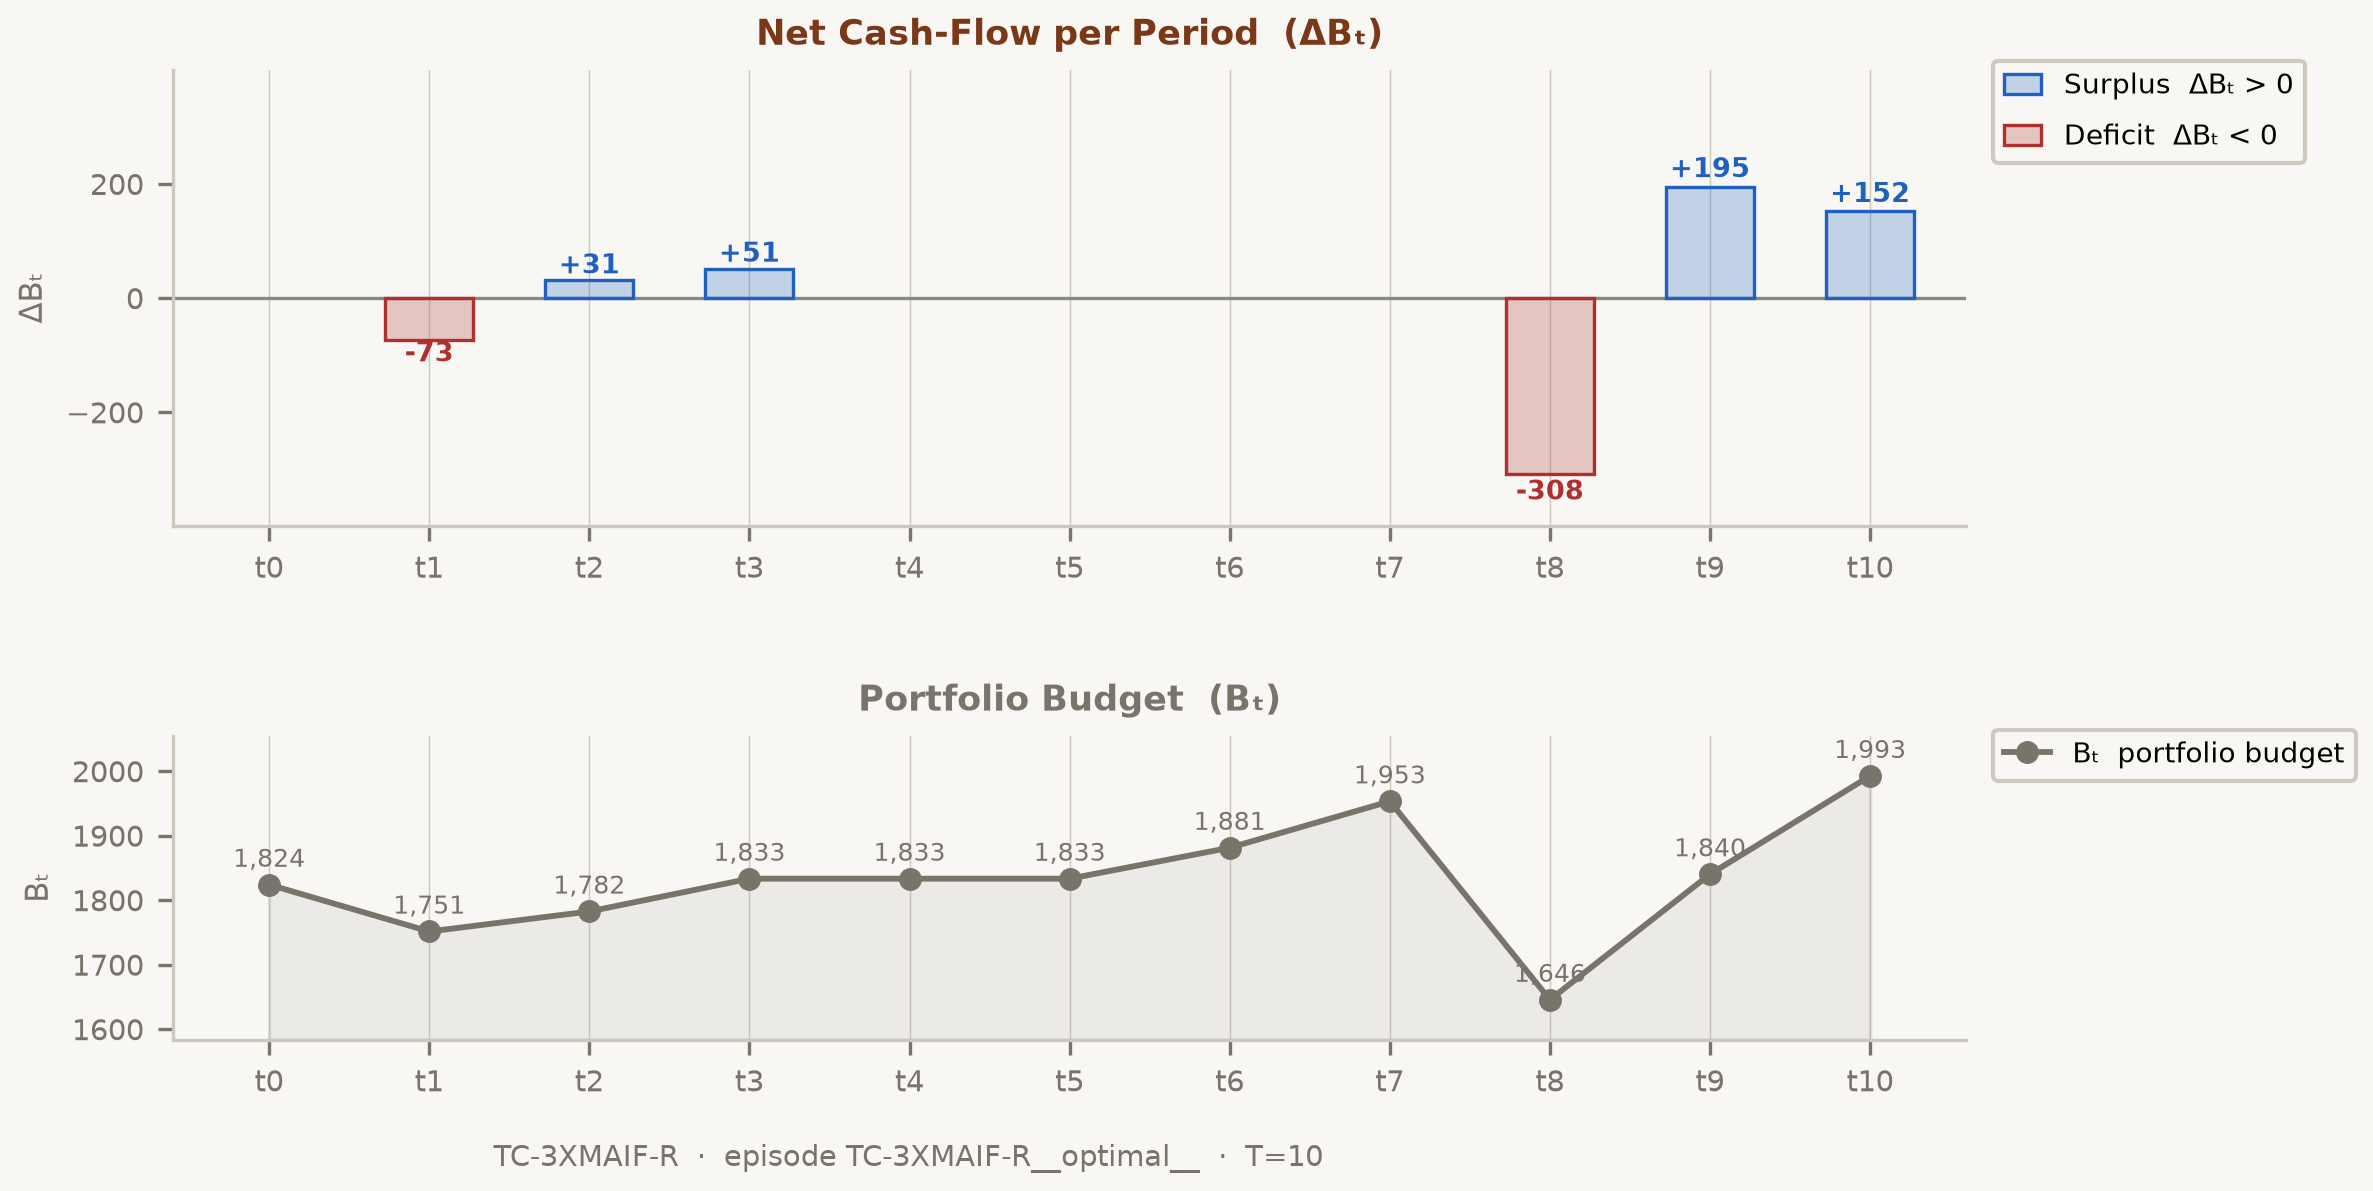
\includegraphics[width=\textwidth]{figures/cashflow_optimal.png}
  \caption[Portfolio Net Cash Flow]{Period-by-period net cash flow
    under $\pi^*$.}
  \label{fig:cashflow_optimal}
\end{figure}

\paragraph{Observation trace.}
Table~\ref{tab:obs_trace} records the full observation vector
$o_t = (B_t,\, \delta_{i,t},\, EV_{i,t},\, \mathrm{breach}_{i,t},\, \ldots)$
at each episode period under $\pi^*$, drawn directly from the SQLite
audit ledger. The table enables verification that breach flags,
advance triggers, and termination conditions are correctly evaluated
by the environment at each step.

\begin{table}[H]
  \centering
  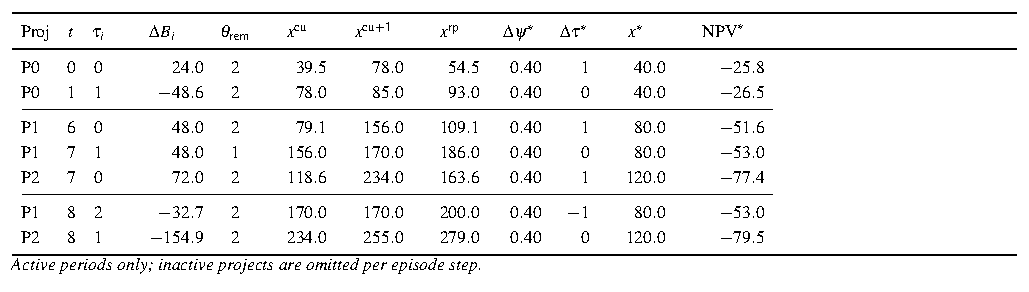
\includegraphics[width=\textwidth]{tables/obs_trace.pdf}
  \caption[Observation Traceback]{Agent observation vector $o_t$
    at each active period under the full-information optimum
    $\pi^*$, drawn from the SQLite audit ledger.}
  \label{tab:obs_trace}
\end{table}

\paragraph{Reward decomposition.}
Table~\ref{tab:reward_trace} decomposes the per-period reward signal
$r_t = \gamma^t \Delta B_t$ into its contributing events: allocation
cost, advance inflow or outflow, milestone payment (gross), recovery
deduction, retention deduction, retention release, and interest
accrual. The final column accumulates the discounted sum $G_t =
\sum_{\tau=0}^{t} \gamma^\tau \Delta B_\tau$, converging to $G =
+12.40$ at episode end.

\begin{table}[H]
  \centering
  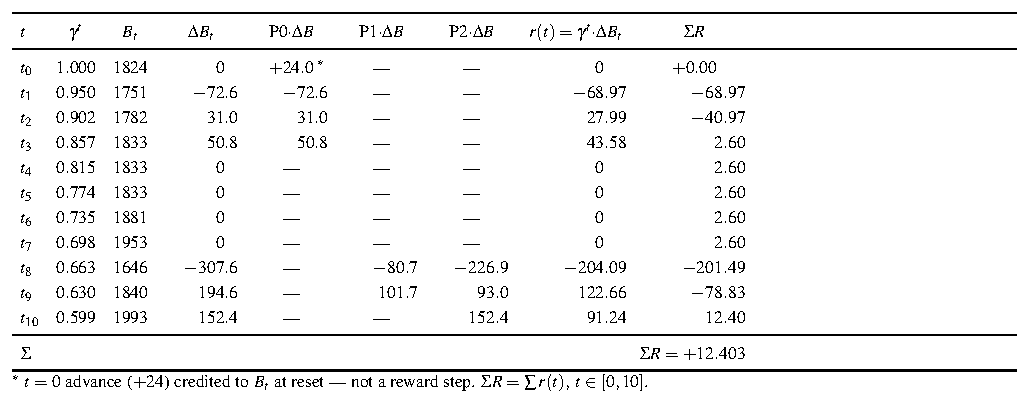
\includegraphics[width=\textwidth]{tables/reward_trace.pdf}
  \caption[Reward Traceback]{Per-period reward decomposition under
    $\pi^*$: signed cash-flow contribution of each event class and
    cumulative discounted return $G_t$.}
  \label{tab:reward_trace}
\end{table}

% ------------------------------------------------------------
\subsection{Results}
\label{subsec:results}
% ------------------------------------------------------------

Figure~\ref{fig:gap_plot} reports cumulative episode NPV $G =
\sum_{t=0}^{T} \gamma^t \Delta B_t$ for each method across the four
configurations, ordered by increasing structural complexity.

\paragraph{TC-10SF-R.}
On the isolated single-period configuration all three heuristics
produce positive NPV and the gap is modest. Reach-Plan achieves
$5.60$ against the optimum $9.00$ (gap $3.40$); Catchup-T follows
at $3.40$. Catchup-Next-T finishes at $-6.07$: with only one active
period and one milestone, its one-period lookahead over-spends
relative to what the milestone requires, incurring interest costs
without a compensating return. The result confirms that the
environment correctly prices conservative over-allocation as a net
loss.

\paragraph{TC-1LMAIF-R.}
The progress-triggered advance and high recovery rate ($\rho_i =
0.50$) create a liquidity trough immediately after the advance fires.
All three heuristics produce negative NPV while the optimum remains
marginally positive at $1.49$; the best-heuristic gap is $14.70$.
The full-information optimum exploits the known efficiency sequence
to time milestone certifications so that the advance trigger fires
at the most advantageous moment and the large recovery deductions at
$j = 1$ ($-9.0$) and $j = 2$ ($-15.0$) are offset by subsequent
cash inflows. The greedy policies, allocating from current-period
signals only, cannot anticipate the trigger timing and over-allocate
during the low-return period before the advance fires. Both
$\pi^{\mathrm{rp}}$ and $\pi^{\mathrm{cu}}$ achieve identical NPV
($-13.21$), indicating that the binding constraint is payment timing
rather than the delay cap.

\paragraph{TC-10MAIF-R.}
The monotonically diminishing efficiency sequence makes the
allocation timing problem acute. Even the full-information optimum
achieves only $-21.66$: the late-stage efficiency collapse
($\eta_{i,t} = 0.30,\, 0.20$) makes full project recovery
uneconomical. Catchup-Next-T ($-27.22$) outperforms both Reach-Plan
($-35.06$) and Catchup-T ($-47.77$): its risk-averse lookahead
front-loads work into the high-efficiency early periods, reducing
expenditure in the near-inoperable late periods. Catchup-T performs
worst because its minimum-spend rule continues allocating into
low-efficiency periods to maintain the tolerance floor, accumulating
cost without meaningful progress. The best-heuristic gap of $5.56$ is
the smallest in the suite, because the challenge here is project-level
efficiency timing rather than multi-project coordination.

\paragraph{TC-3XMAIF-R.}
The multi-project configuration produces the starkest result. The
full-information optimum achieves $+12.40$: with known efficiency
sequences, the oracle times advance disbursements, milestone
certifications, and the gap-phase budget accumulation to convert the
complex portfolio into a profitable episode. Every greedy heuristic
produces a loss --- Reach-Plan at $-59.75$, Catchup-T at $-62.38$,
Catchup-Next-T at $-107.96$ --- and the best-heuristic gap reaches
$72.15$, a $21\times$ increase over TC-10SF-R. The sign reversal
(profitable optimum, loss-making heuristics) is the central
observation. The concurrent advance outflows at $t = 6$ ($-48$) and
$t = 7$ ($-72$) create a large shared deficit that each single-project
greedy rule handles independently, without accounting for how its own
allocation depletes the reserve available to the concurrent project.
Catchup-Next-T collapses to $-107.96$ because its aggressive
pre-emptive spend across all three simultaneously-active projects
exhausts the budget during the overlap phase, leaving insufficient
reserve to certify the high-value late milestones of Projects~1 and 2.

\begin{figure}[H]
  \centering
  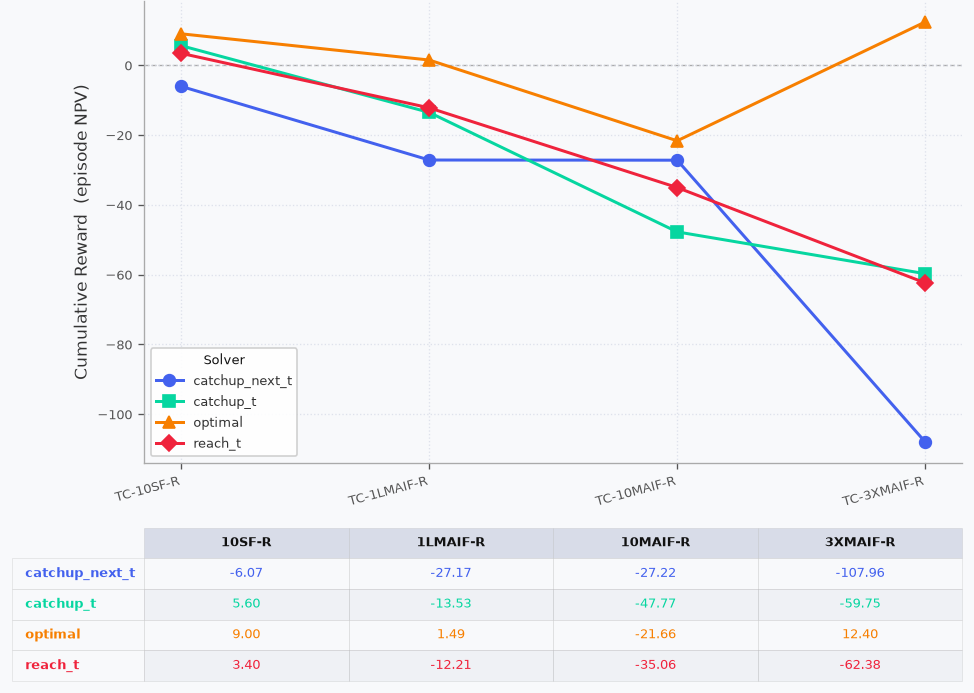
\includegraphics[width=\textwidth]{figures/gap_plot.png}
  \caption[Optimality Gap]{Episode NPV by configuration and solver;
    gap widens monotonically with structural complexity.}
  \label{fig:gap_plot}
\end{figure}

% ------------------------------------------------------------
\subsection{Discussion}
\label{subsec:discussion}
% ------------------------------------------------------------

Three findings emerge from the benchmark study.

\paragraph{The gap is monotonically increasing with structural
complexity.}
The best-heuristic gap grows from $3.40$ (TC-10SF-R) to $14.70$
(TC-1LMAIF-R) to $72.15$ (TC-3XMAIF-R), a $21\times$ increase from
simplest to most complex. TC-10MAIF-R ($5.56$) is the only departure
from strict monotonicity: its challenge is project-level efficiency
timing, not multi-project coordination, so the gap is smaller than
TC-1LMAIF-R's despite higher individual-project difficulty. The gap
in TC-3XMAIF-R is not marginal degradation; it reflects a structural
failure of greedy allocation under shared-budget coordination
requirements that no single-project rule can resolve.

\paragraph{No single heuristic dominates.}
Each heuristic is best on at least one configuration: Reach-Plan on
TC-10SF-R, Catchup-Next-T on TC-10MAIF-R, Catchup-T on TC-3XMAIF-R.
This confirms that the optimal policy is adaptive: the correct
allocation depends jointly on the efficiency trajectory, the milestone
payment structure, the advance trigger timing, and the phasing of
concurrent projects --- a combination no fixed rule can capture.
The failure mode of each heuristic is traceable to a specific
structural feature: Reach-Plan over-spends in aggregate; Catchup-T
under-anticipates the lookahead; Catchup-Next-T over-commits in the
multi-project overlap phase.

\paragraph{A well-defined improvement target exists for learned agents.}
The full-information optimum $G(\pi^*)$ provides a concrete upper
bound (Proposition~\ref{prop:upper_bound}) for each configuration.
On TC-3XMAIF-R the swing between the best achievable ($+12.40$) and
the best greedy ($-59.75$) is $72.15$ NPV units --- the difference
between a profitable and a deeply loss-making portfolio outcome. The
environment mechanics are thereby empirically validated: each
configuration produces the expected pattern of cash-flow events
(advance disbursements, milestone certifications, recovery deductions,
retention release, interest accrual) correctly sequenced and
financially consistent, and the full-information optimum exploits
structural features that greedy rules are architecturally unable to
access. This gap constitutes the performance target for future RL
agents trained on the environment of Section~\ref{sec:problem}.